\section{Vernier Calipers}
\label{vernier_caliper}

A vernier is a small auxiliary scale that slides along the main scale. It allows more accurate estimates of fractional parts of the smallest division on the main scale.

On a vernier caliper, the main scale is engraved on the fixed part of the instrument. The vernier scale, engraved on the movable jaw, has ten divisions that cover the same spatial interval as nine divisions on the main scale: each vernier division is $\frac{9}{10}$ the length of a main scale division. 
%In the case of a vernier caliper, the vernier division length is 0.9 mm. 

\begin{center}
\medskip
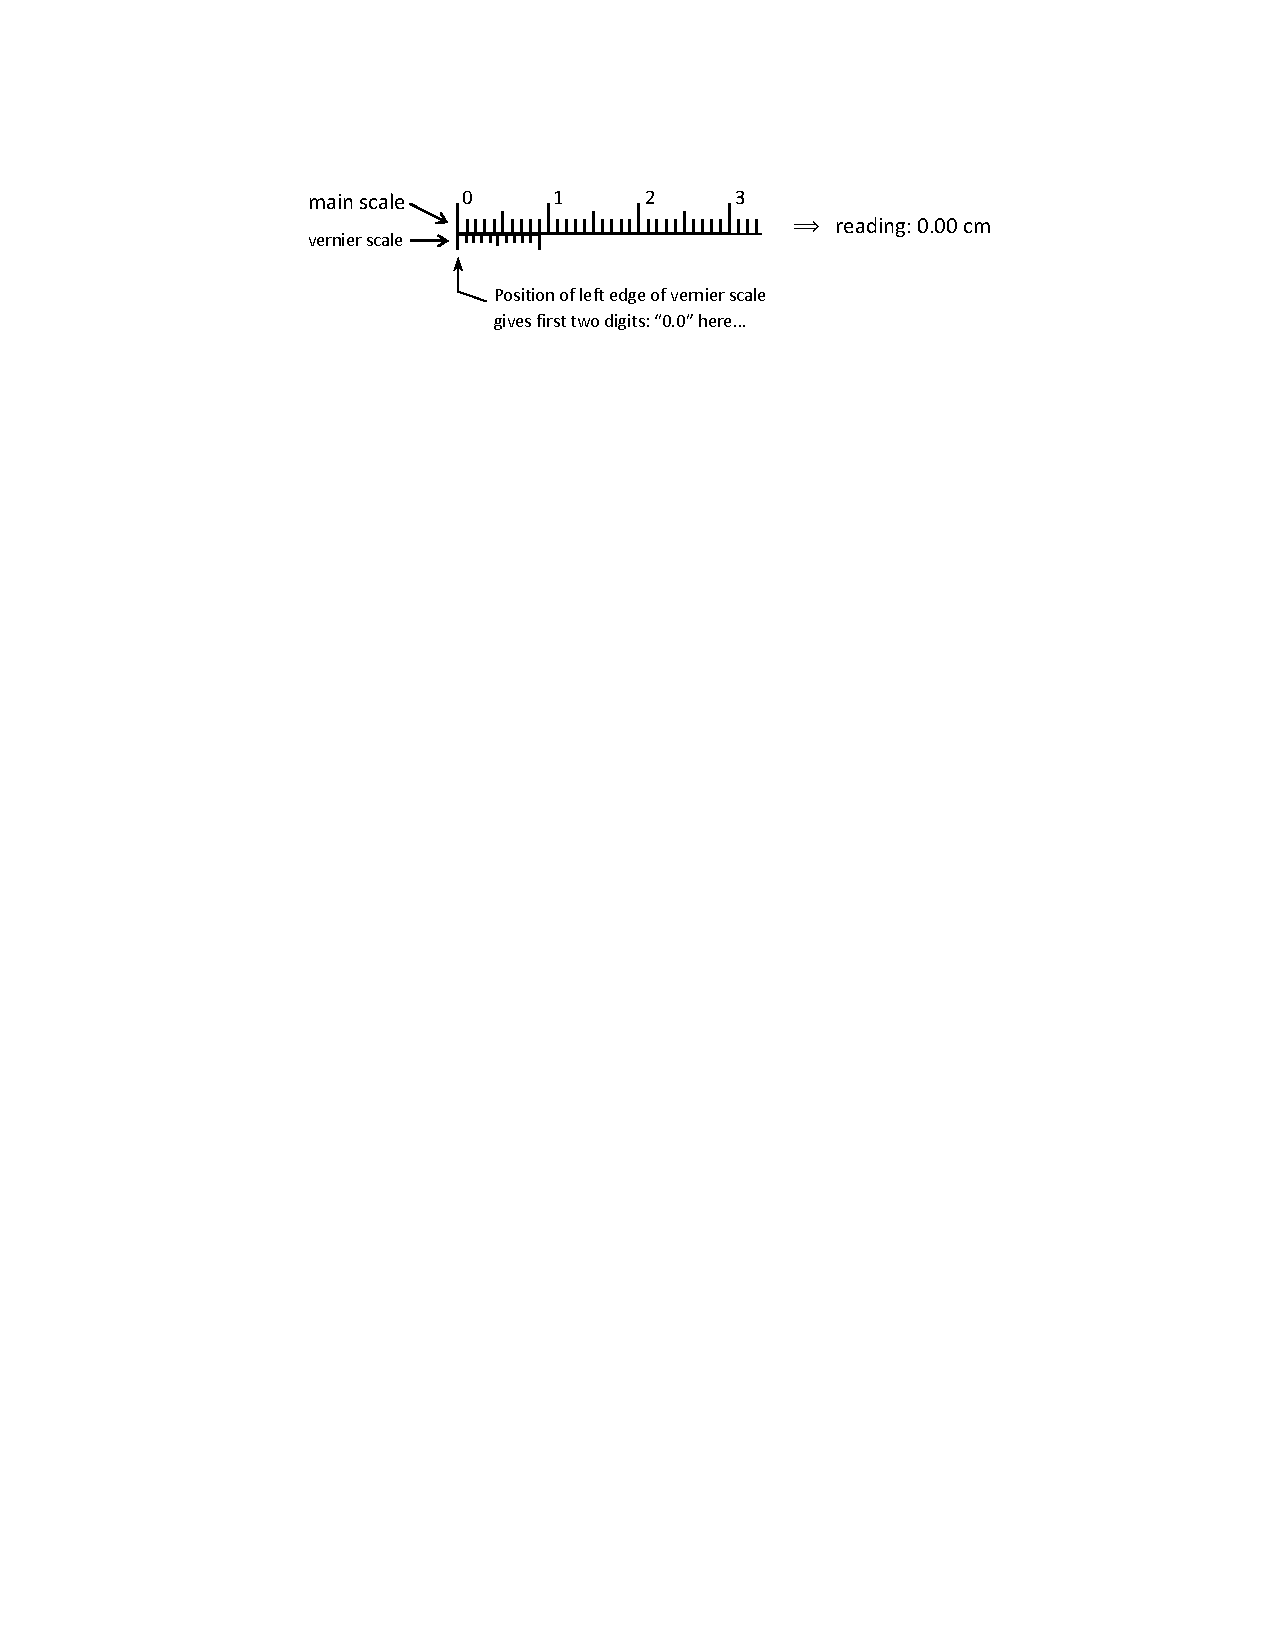
\includegraphics{appendices/instrumentation/vernier_0p0_cm.pdf}

\vspace{0.1in}
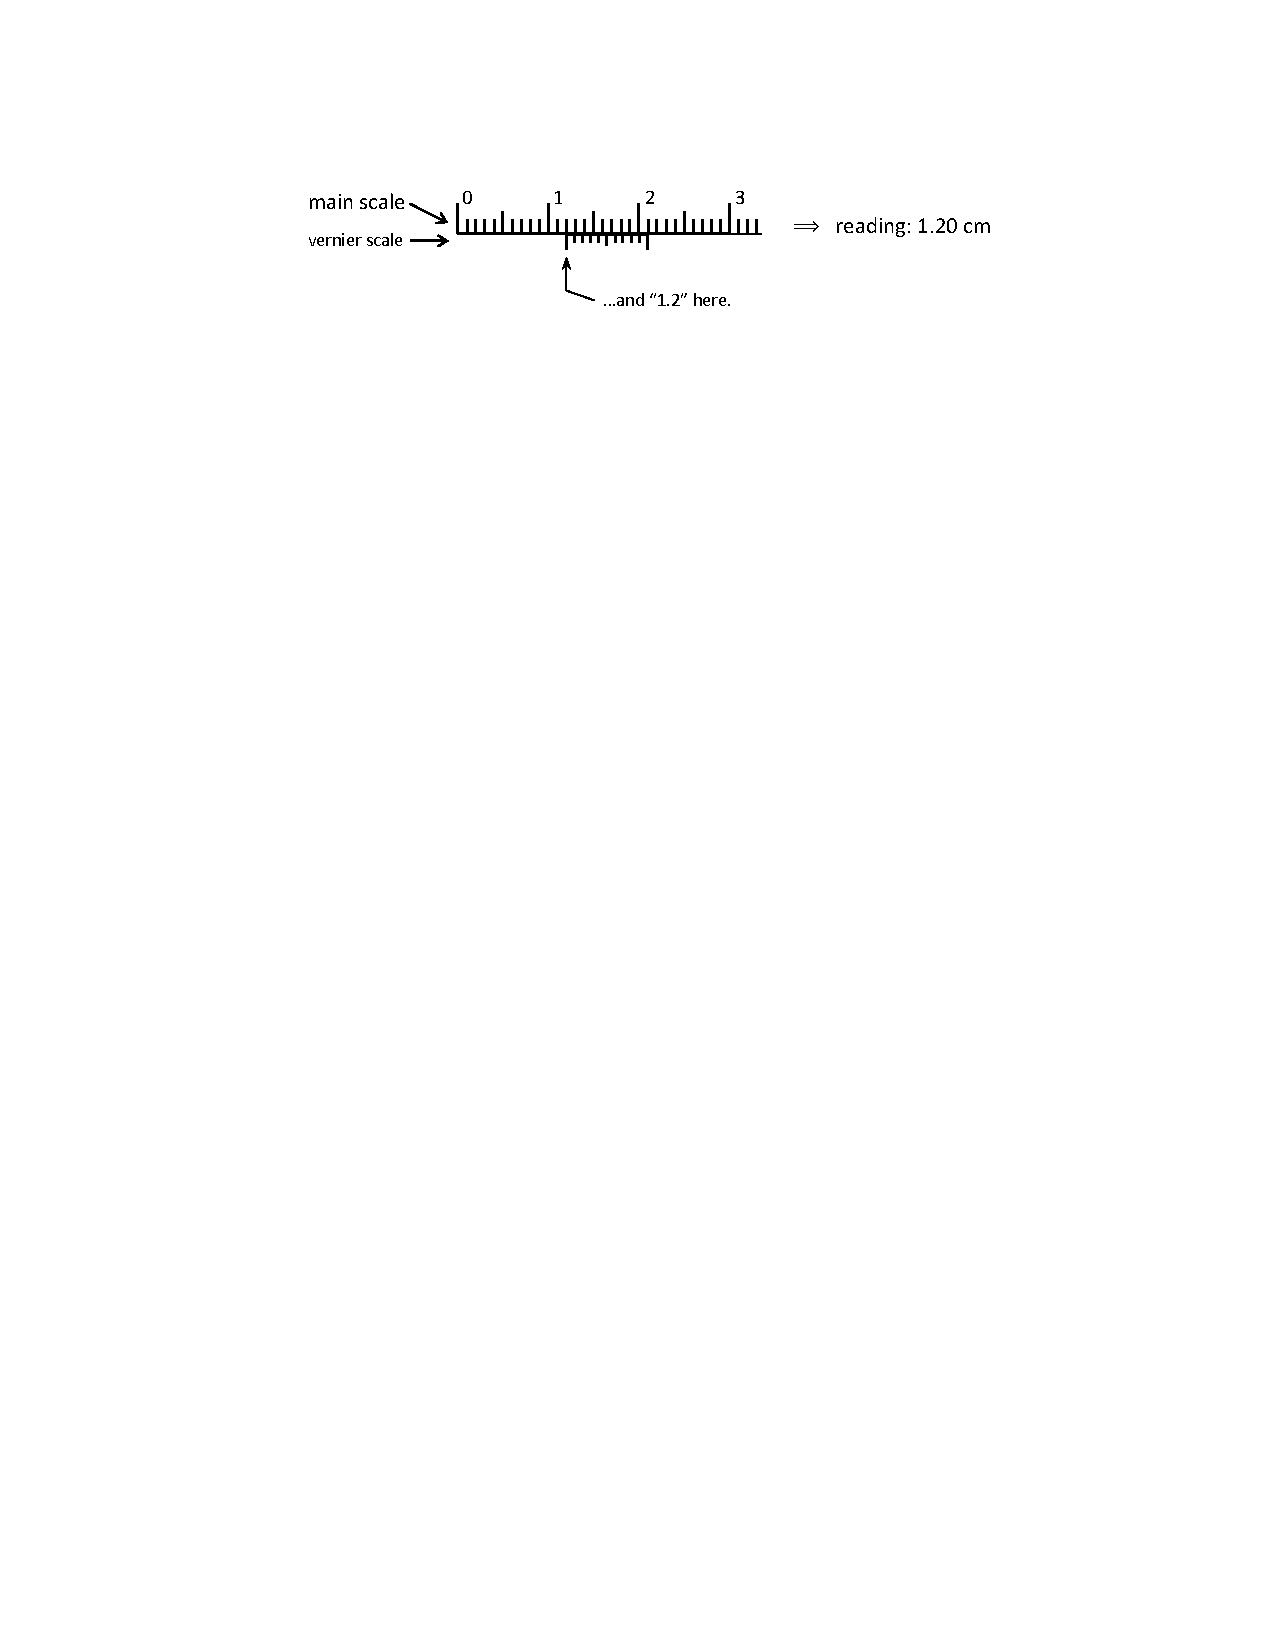
\includegraphics{appendices/instrumentation/vernier_1p2_cm.pdf}

\vspace{0.1in}
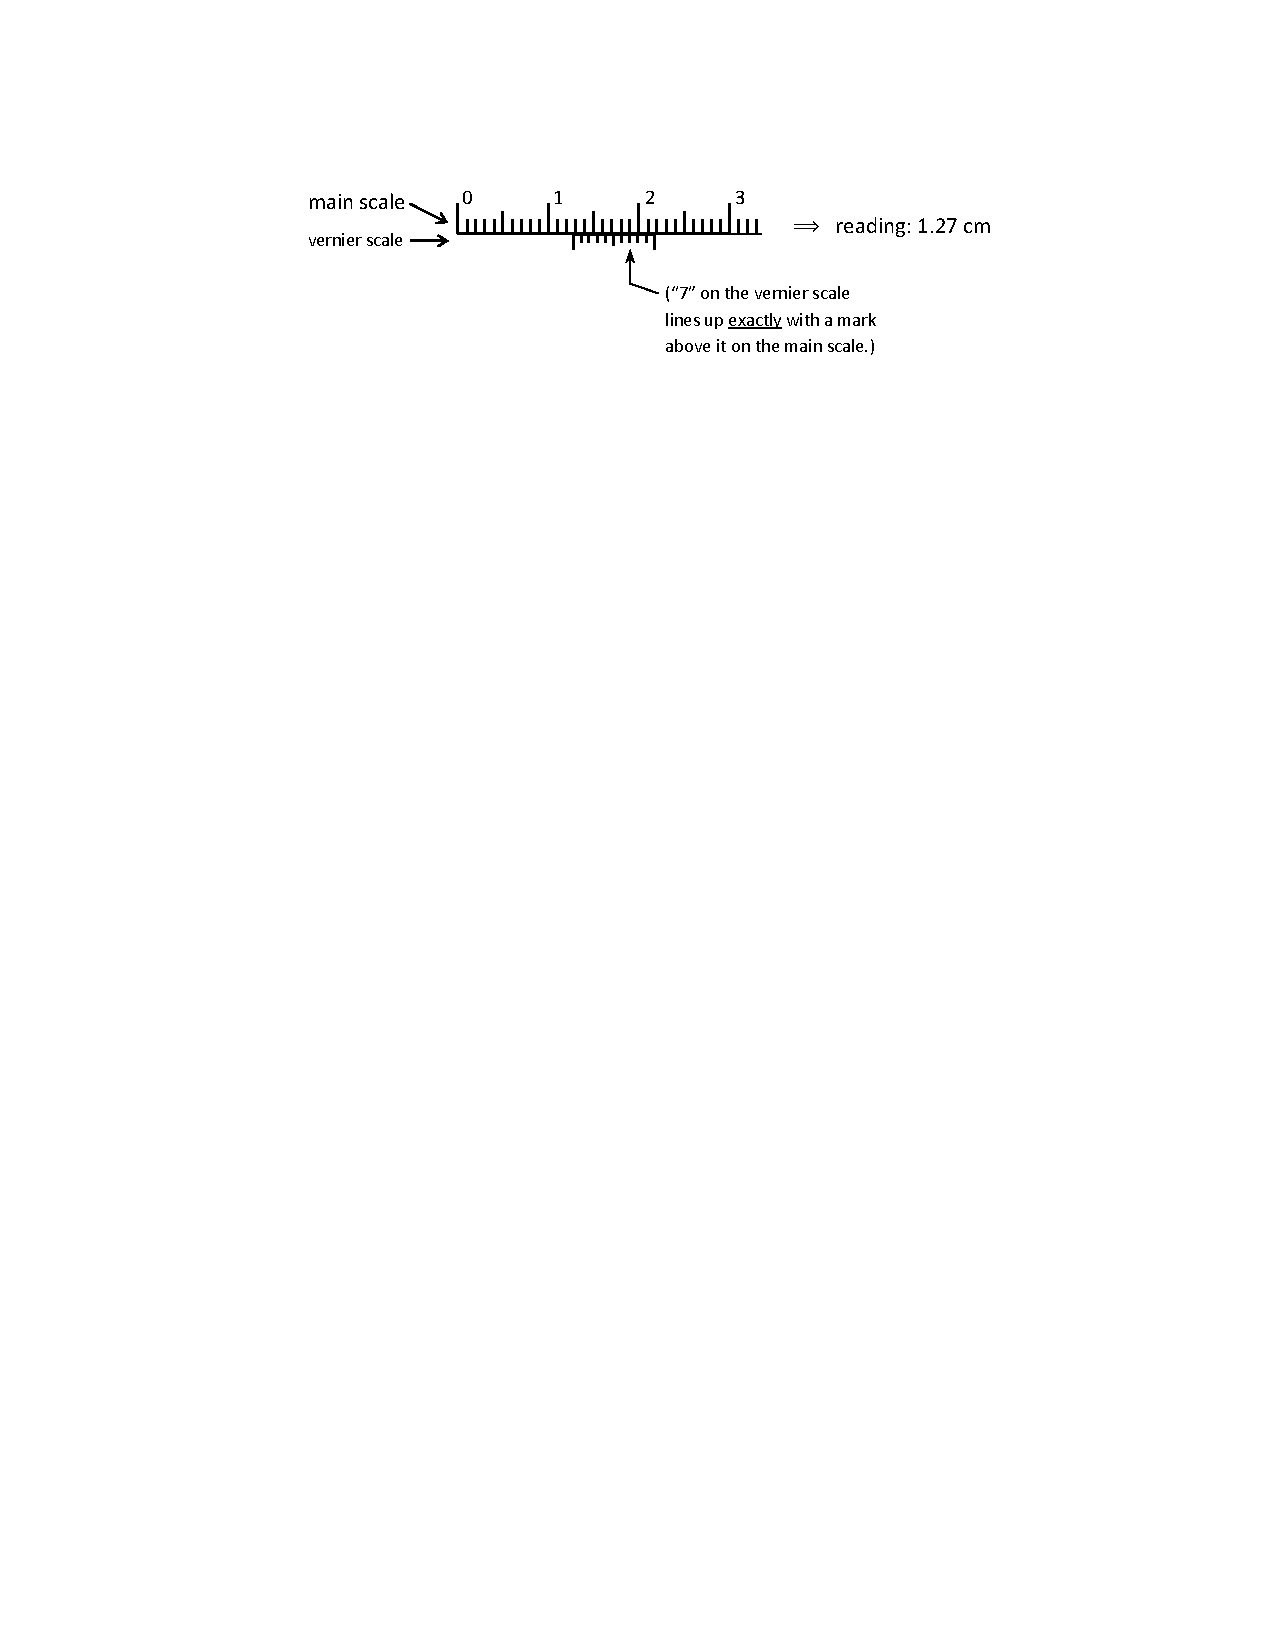
\includegraphics{appendices/instrumentation/vernier_1p27_cm.pdf}
\end{center} 

\medskip

To measure length with a vernier caliper, close the jaws on the object and read the two scales.
\begin{itemize}
\item The first digit is read from the main scale.  Look at where the left-most edge of the vernier scale lines up with the main scale, and read the digit from the main scale.  

\begin{quote}
\textit{In the top example above, the first digit is ``0''.  
In the second and third examples, it's ``1''.}
\end{quote}
\item The second digit is also read from the main scale.  Again, look at where the left-most edge of the vernier scale lines up, and read the closest subdivision from the main scale.  

\begin{quote}
\textit{In the second and third examples above, the second digit is ``2''.}
\end{quote}

\item The third digit is read from the vernier scale.  Read which mark on the vernier scale lines up \textit{exactly} with a mark above it on the main scale. 

\begin{quote}
\textit{In the third example, it's clear that the left edge of the vernier scale is a little above 1.2 on the main scale, but it's hard to tell from the main scale exactly what the third digit is.  (Maybe 1.25? or 1.26?)  But look at the marks on the vernier scale: the 6 and 8 don't quite line up with any marks on the main scale, but the 7 lines up exactly, so the last digit is ``7''.}
\end{quote}
\end{itemize}

If the zero lines of the main and vernier scales do not align when the jaws are closed, all measurements will be systematically shifted. The magnitude of this shift, called the zero reading or zero correction, should be noted and recorded, so that length measurements made with the vernier caliper can be corrected, thereby removing the systematic error.

